

\tikzset{every picture/.style={line width=0.75pt}} %

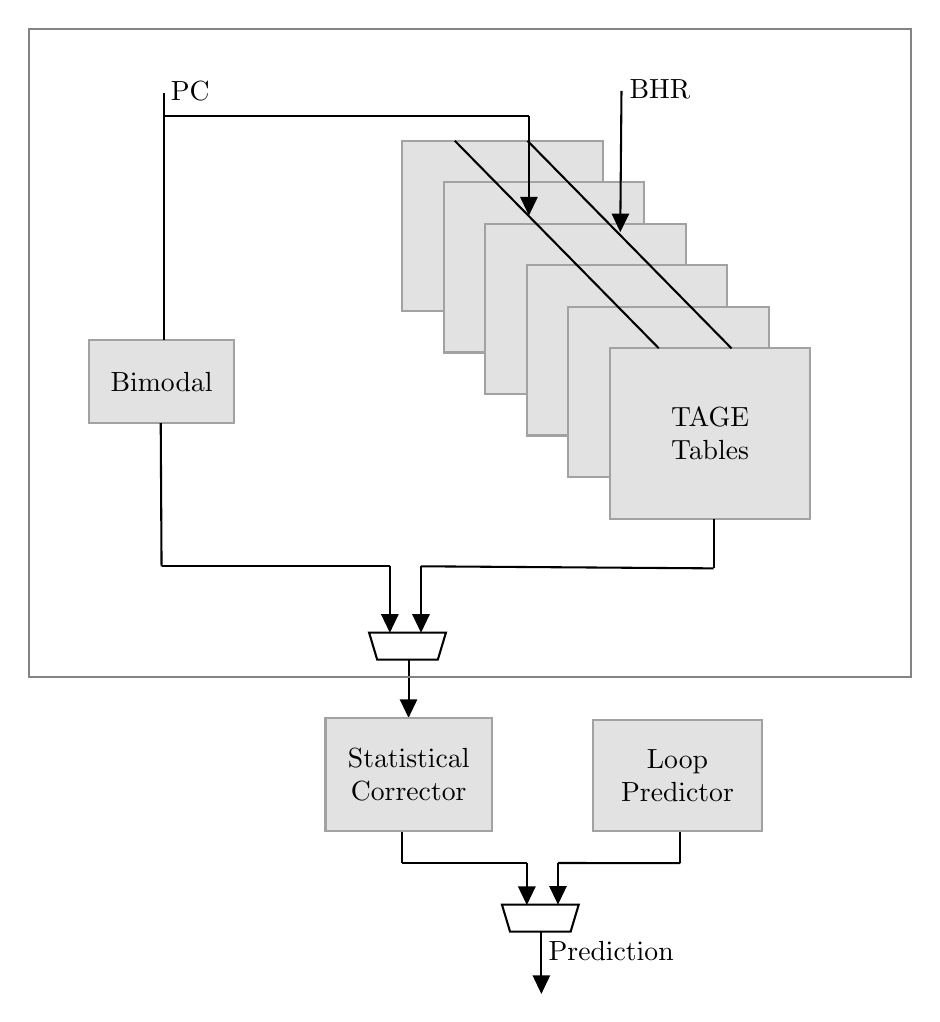
\begin{tikzpicture}[x=0.75pt,y=0.75pt,yscale=-1,xscale=1]

\draw  [color={rgb, 255:red, 162; green, 162; blue, 162 }  ,draw opacity=1 ][fill={rgb, 255:red, 226; green, 226; blue, 226 }  ,fill opacity=1 ] (149,328) -- (219,328) -- (219,368) -- (149,368) -- cycle ;
\draw    (185,209) -- (185,328) ;
\draw    (183.6,368) -- (184,437) ;
\draw  [color={rgb, 255:red, 162; green, 162; blue, 162 }  ,draw opacity=1 ][fill={rgb, 255:red, 226; green, 226; blue, 226 }  ,fill opacity=1 ] (300,232) -- (396.6,232) -- (396.6,314) -- (300,314) -- cycle ;
\draw  [color={rgb, 255:red, 162; green, 162; blue, 162 }  ,draw opacity=1 ][fill={rgb, 255:red, 226; green, 226; blue, 226 }  ,fill opacity=1 ] (320,252) -- (416.6,252) -- (416.6,334) -- (320,334) -- cycle ;
\draw  [color={rgb, 255:red, 162; green, 162; blue, 162 }  ,draw opacity=1 ][fill={rgb, 255:red, 226; green, 226; blue, 226 }  ,fill opacity=1 ] (340,272) -- (436.6,272) -- (436.6,354) -- (340,354) -- cycle ;
\draw  [color={rgb, 255:red, 162; green, 162; blue, 162 }  ,draw opacity=1 ][fill={rgb, 255:red, 226; green, 226; blue, 226 }  ,fill opacity=1 ] (360,292) -- (456.6,292) -- (456.6,374) -- (360,374) -- cycle ;
\draw  [color={rgb, 255:red, 162; green, 162; blue, 162 }  ,draw opacity=1 ][fill={rgb, 255:red, 226; green, 226; blue, 226 }  ,fill opacity=1 ] (380,312) -- (476.6,312) -- (476.6,394) -- (380,394) -- cycle ;
\draw  [color={rgb, 255:red, 162; green, 162; blue, 162 }  ,draw opacity=1 ][fill={rgb, 255:red, 226; green, 226; blue, 226 }  ,fill opacity=1 ] (400,332) -- (496.6,332) -- (496.6,414) -- (400,414) -- cycle ;
\draw    (325.3,232) -- (423.6,332) ;
\draw    (360.3,232) -- (458.6,332) ;
\draw    (361,220) -- (361,265) ;
\draw [shift={(361,268)}, rotate = 270] [fill={rgb, 255:red, 0; green, 0; blue, 0 }  ][line width=0.08]  [draw opacity=0] (8.93,-4.29) -- (0,0) -- (8.93,4.29) -- cycle    ;
\draw    (185,220) -- (361,220) ;
\draw    (405.6,208) -- (405.03,273) ;
\draw [shift={(405,276)}, rotate = 270.51] [fill={rgb, 255:red, 0; green, 0; blue, 0 }  ][line width=0.08]  [draw opacity=0] (8.93,-4.29) -- (0,0) -- (8.93,4.29) -- cycle    ;
\draw    (184,437) -- (294,437) ;
\draw    (294,437) -- (294,466) ;
\draw [shift={(294,469)}, rotate = 270] [fill={rgb, 255:red, 0; green, 0; blue, 0 }  ][line width=0.08]  [draw opacity=0] (8.93,-4.29) -- (0,0) -- (8.93,4.29) -- cycle    ;
\draw    (309,437) -- (309,466) ;
\draw [shift={(309,469)}, rotate = 270] [fill={rgb, 255:red, 0; green, 0; blue, 0 }  ][line width=0.08]  [draw opacity=0] (8.93,-4.29) -- (0,0) -- (8.93,4.29) -- cycle    ;
\draw    (309,437) -- (450,438) ;
\draw    (450,414) -- (450,438) ;
\draw   (321,469) -- (317.1,482) -- (287.9,482) -- (284,469) -- cycle ;
\draw    (303,482) -- (303,507) ;
\draw [shift={(303,510)}, rotate = 270] [fill={rgb, 255:red, 0; green, 0; blue, 0 }  ][line width=0.08]  [draw opacity=0] (8.93,-4.29) -- (0,0) -- (8.93,4.29) -- cycle    ;
\draw  [color={rgb, 255:red, 131; green, 131; blue, 131 }  ,draw opacity=1 ] (120,178) -- (545.13,178) -- (545.13,490.47) -- (120,490.47) -- cycle ;
\draw  [color={rgb, 255:red, 162; green, 162; blue, 162 }  ,draw opacity=1 ][fill={rgb, 255:red, 226; green, 226; blue, 226 }  ,fill opacity=1 ] (392,511) -- (473.13,511) -- (473.13,564.47) -- (392,564.47) -- cycle ;
\draw  [color={rgb, 255:red, 162; green, 162; blue, 162 }  ,draw opacity=1 ][fill={rgb, 255:red, 226; green, 226; blue, 226 }  ,fill opacity=1 ] (263,510) -- (343.13,510) -- (343.13,564.47) -- (263,564.47) -- cycle ;
\draw    (300,580) -- (360,580) ;
\draw    (360,580) -- (360,597.2) ;
\draw [shift={(360,600.2)}, rotate = 270] [fill={rgb, 255:red, 0; green, 0; blue, 0 }  ][line width=0.08]  [draw opacity=0] (8.93,-4.29) -- (0,0) -- (8.93,4.29) -- cycle    ;
\draw    (375,579.95) -- (375,597) ;
\draw [shift={(375,600)}, rotate = 270] [fill={rgb, 255:red, 0; green, 0; blue, 0 }  ][line width=0.08]  [draw opacity=0] (8.93,-4.29) -- (0,0) -- (8.93,4.29) -- cycle    ;
\draw    (375,579.95) -- (434,580.04) ;
\draw    (434,565) -- (434,580.04) ;

\draw    (300,564.93) -- (300,580) ;
\draw   (385,600) -- (381.1,613) -- (351.9,613) -- (348,600) -- cycle ;
\draw    (367,613) -- (367,640) ;
\draw [shift={(367,643)}, rotate = 270] [fill={rgb, 255:red, 0; green, 0; blue, 0 }  ][line width=0.08]  [draw opacity=0] (8.93,-4.29) -- (0,0) -- (8.93,4.29) -- cycle    ;


\draw (187,202) node [anchor=north west][inner sep=0.75pt]   [align=left] {\textbf{{\fontfamily{helvet}\selectfont PC}}};
\draw (408,201) node [anchor=north west][inner sep=0.75pt]   [align=left] {\textbf{{\fontfamily{helvet}\selectfont BHR}}};
\draw (369,616) node [anchor=north west][inner sep=0.75pt]   [align=left] {\textbf{{\fontfamily{helvet}\selectfont Prediction}}};
\draw (184,348) node   [align=left] {\textbf{{\fontfamily{helvet}\selectfont Bimodal}}};
\draw (303.07,537.23) node   [align=left] {\begin{minipage}[lt]{50.92pt}\setlength\topsep{0pt}
\begin{center}
\textbf{{\fontfamily{helvet}\selectfont Statistical}}\\\textbf{{\fontfamily{helvet}\selectfont Corrector}}
\end{center}

\end{minipage}};
\draw (432.57,537.73) node   [align=left] {\begin{minipage}[lt]{47.5pt}\setlength\topsep{0pt}
\begin{center}
\textbf{{\fontfamily{helvet}\selectfont Loop}}\\\textbf{{\fontfamily{helvet}\selectfont Predictor}}
\end{center}

\end{minipage}};
\draw (448.3,373) node   [align=left] {\begin{minipage}[lt]{34.28pt}\setlength\topsep{0pt}
\begin{center}
\textbf{{\fontfamily{helvet}\selectfont TAGE}}\\\textbf{{\fontfamily{helvet}\selectfont Tables}}
\end{center}

\end{minipage}};


\end{tikzpicture}
